%%
%% This is file `sample-lualatex.tex',
%% generated with the docstrip utility.
%%
%% The original source files were:
%%
%% samples.dtx  (with options: `sigconf')
%% 
%% IMPORTANT NOTICE:
%% 
%% For the copyright see the source file.
%% 
%% Any modified versions of this file must be renamed
%% with new filenames distinct from sample-lualatex.tex.
%% 
%% For distribution of the original source see the terms
%% for copying and modification in the file samples.dtx.
%% 
%% This generated file may be distributed as long as the
%% original source files, as listed above, are part of the
%% same distribution. (The sources need not necessarily be
%% in the same archive or directory.)
%%
%% The first command in your LaTeX source must be the \documentclass command.
\documentclass[sigconf]{acmart}
%% NOTE that a single column version is required for 
%% submission and peer review. This can be done by changing
%% the \doucmentclass[...]{acmart} in this template to 
%% \documentclass[manuscript,screen]{acmart}
%% 
%% To ensure 100% compatibility, please check the white list of
%% approved LaTeX packages to be used with the Master Article Template at
%% https://www.acm.org/publications/taps/whitelist-of-latex-packages 
%% before creating your document. The white list page provides 
%% information on how to submit additional LaTeX packages for 
%% review and adoption.
%% Fonts used in the template cannot be substituted; margin 
%% adjustments are not allowed.

%%
%% \BibTeX command to typeset BibTeX logo in the docs
\AtBeginDocument{%
  \providecommand\BibTeX{{%
    \normalfont B\kern-0.5em{\scshape i\kern-0.25em b}\kern-0.8em\TeX}}}

%% Rights management information.  This information is sent to you
%% when you complete the rights form.  These commands have SAMPLE
%% values in them; it is your responsibility as an author to replace
%% the commands and values with those provided to you when you
%% complete the rights form.
\setcopyright{acmcopyright}
\copyrightyear{2022}
\acmYear{2022}
\acmDOI{XXXXXXX.XXXXXXX}

%% Add images folder as source for graphics
\graphicspath{ {images/} }

%% These commands are for a PROCEEDINGS abstract or paper.
\acmConference[Conference acronym 'XX]{Make sure to enter the correct
  conference title from your rights confirmation emai}{June 03--05,
  2018}{Woodstock, NY}
%
%  Uncomment \acmBooktitle if th title of the proceedings is different
%  from ``Proceedings of ...''!
%
%\acmBooktitle{Woodstock '18: ACM Symposium on Neural Gaze Detection,
%  June 03--05, 2018, Woodstock, NY} 
\acmPrice{15.00}
\acmISBN{978-1-4503-XXXX-X/18/06}


%%
%% Submission ID.
%% Use this when submitting an article to a sponsored event. You'll
%% receive a unique submission ID from the organizers
%% of the event, and this ID should be used as the parameter to this command.
%%\acmSubmissionID{123-A56-BU3}

%%
%% The majority of ACM publications use numbered citations and
%% references.  The command \citestyle{authoryear} switches to the
%% "author year" style.
%%
%% If you are preparing content for an event
%% sponsored by ACM SIGGRAPH, you must use the "author year" style of
%% citations and references.
%% Uncommenting
%% the next command will enable that style.
%%\citestyle{acmauthoryear}

%%
%% end of the preamble, start of the body of the document source.

\begin{document}

%%
%% The "title" command has an optional parameter,
%% allowing the author to define a "short title" to be used in page headers.
\title{Master Thesis Proposal: Risk detection and risk control through sprint backlog analysis}

%%
%% The "author" command and its associated commands are used to define
%% the authors and their affiliations.
%% Of note is the shared affiliation of the first two authors, and the
%% "authornote" and "authornotemark" commands
%% used to denote shared contribution to the research.
\author{Sytse Groenwold}
\affiliation{13083228}
\email{sytse.groenwold@student.uva.nl}

\author{Zhiming Zhao}
\affiliation{Supervisor}
\email{z.zhao@uva.nl}

\author{TBD}
\affiliation{Examiner}
\email{email}

%%
%% By default, the full list of authors will be used in the page
%% headers. Often, this list is too long, and will overlap
%% other information printed in the page headers. This command allows
%% the author to define a more concise list
%% of authors' names for this purpose.
\renewcommand{\shortauthors}{Groenwold, S.}

%%
%% The abstract is a short summary of the work to be presented in the
%% article.
\begin{abstract}

DISCLAIMER: 

Find the most recent version of my design through GitHub: \url{https://github.com/SytseGroenwold/masters-thesis}. I would immensely appreciate it if you can take the lastest version from there when providing feedback; I plan to finalise it by Sunday 27th of February, but I understand if you cannot wait until then. \\

I have only secured this project 3 weeks ago and only last week the supervisor and I settled on the subject. Hence my paper being in such a raw shape. It speaks for itself which sections are more fleshed out and which are mere summations of points I wish to talk about. I would greatly appreciate it if you can take this into account while reviewing it.
\end{abstract}

%%
%% Keywords. The author(s) should pick words that accurately describe
%% the work being presented. Separate the keywords with commas.
\keywords{Agile, Scrum, Risk, User Stories, Sprint Backlog, Machine Learning}

%%
%% This command processes the author and affiliation and title
%% information and builds the first part of the formatted document.
\maketitle

\section{Introduction}
In software development, there are several risk events that can decrease product quality, delay delivery or even cause the project to fail[2]. 
Tangible examples of these events are budget overruns and losing personnel, while more subtle ones include a lack of clearly defining work to be done or team members being unaligned. 
(Early) detection (i.e. risk assessment) of such risks and controlling them effectively (i.e. risk control) is crucial for the success of a project[3].

The Agile development methodologies have demonstrated their advantages over traditional methods in reducing time to market, overall product quality and a closer alignment to business needs[5]. 
In Scrum, this is achieved through an iterative process over a short period of time, called sprints. The product manager creates a backlog of user stories, which are the business requirements translated to work for the development team. 
During a sprint, the team works on a selected number of these user stories and afterwards they reflect on both the work done and the collaboration within the team.
Despite these improvements, Agile methodologies can still suffer from risks such as unclear user stories, inefficient decomposition, and scheduling of the sprint backlogs. 
Determining those risk through analysis of the user stories in the product backlog is mostly done by human experts. 
In a previous study, we sought to automate this process, by creating an machine learning model based on previous works and ensembling those models. 

While those results show promise for a machine learning model to detect risks, improvement is needed to make the predictions more robust, especially to achieve more consistent scores between different datasets.
We determined that incorporating the sprint plannings, instead of only analysing the individual user stories, could be a valuable addition to the model parameters in achieving this goal. In this study we plan to do that, and additionally investigate a way to single-out the specific risks that are inside a sprint backlog, so that teams can exercise risk control before they affect the team output.

\subsection{Research question}
To what extend can inclusion of sprint backlog analysis improve risk assessment within software teams using Scrum and how can this risk assessment lead lead to and improvement of risk control?

\subsection{Sub questions}
These are the sub questions

\section{Exploratory Data Analysis}
Among the different software packages used by Scrum adaptors to track user stories, Jira is by far the most used one, having a large margin over other popular services such as Service-Now, Trello and Azure DevOps.
For this study, due to widescale availability, only data sets extracted from Jira will initially be used. If it turns out that this is insufficient, other data sets can be explored.

The requirements for the data sets are straight-forward: they are collections of user stories that are gathered in both product backlogs and sprint backlogs. Additionally, each user story needs to contain the description the story, the date it was created, the date it is completed, and in which sprints backlogs it has been included.
The sprint backlogs are not even required to be individually gathered: if each user story has a record of the sprints it was part of, it should be sufficient information for the model.

The data sets that will be considered for this study are publicly available data sets, which mostly come from github accounts of other researchers whom have gathered them for previous studies. 
When these data sets prove to not be sufficient, there will be two options to gather a data set from organistations (Utrecht University's internal software development department or ING Bank's data sat of user stories stored in Service Now).
There are previous studies who have already worked with these data sets, but as they are not publicly available and are constantly growing, they will only at at later moment be gathered if there is a necessity for them.
Lastly, this project's supervisor is currently giving a course on DevOps and Cloud-based Software, in which different teams of students will need to work together using a user story backlog. At the end of this course (March), the students are to hand in an overview of their product/sprint backlogs as well and these can be considered for this study.

The model for the data sets gathered from Jira have the following features. In a later stage of the project, features which are not used can be left out.

\begin{table}[h]
\caption{Overview of features in the Jira user story data sets.}
\begin{tabular}{|lll|}
\hline
\multicolumn{1}{|c}{\#} & \multicolumn{1}{c}{Feature} & \multicolumn{1}{c|}{Description}                                                                                     \\ \hline
1                       & Issue id                    & \begin{tabular}[c]{@{}l@{}}Issue is Jira's name for a\\ user story\end{tabular}                                      \\
2                       & Summary                     &                                                                                                                      \\
3                       & Description                 &                                                                                                                      \\
4                       & Status                      &                                                                                                                      \\
5                       & Resolution                  &                                                                                                                      \\
6                       & Project key                 &                                                                                                                      \\
7                       & Priority                    &                                                                                                                      \\
8                       & Rank                        &                                                                                                                      \\
9                       & Impact                      &                                                                                                                      \\
10                      & Votes                       &                                                                                                                      \\
11                      & Story point estimate        &                                                                                                                      \\
12                      & Change reason               &                                                                                                                      \\
13                      & Change risk                 &                                                                                                                      \\
14                      & Change type                 &                                                                                                                      \\
15                      & Request type                &                                                                                                                      \\
16                      & Epic name                   &                                                                                                                      \\
17                      & Environment                 & sbx, dev, tst, acc, prd                                                                                              \\
18                      & Security level              &                                                                                                                      \\
19                      & Assignee ID                 &                                                                                                                      \\
20                      & Reporter ID                 &                                                                                                                      \\
21                      & Creator ID                  &                                                                                                                      \\
22                      & Watchers ID                 &                                                                                                                      \\
23                      & Created                     &                                                                                                                      \\
24                      & Updated                     &                                                                                                                      \\
25                      & Last Viewed                 &                                                                                                                      \\
26                      & Resolved                    &                                                                                                                      \\
27                      & Due date                    &                                                                                                                      \\
28                      & Actual end                  &                                                                                                                      \\
29                      & Actual start                &                                                                                                                      \\
30                      & Original estimate           &                                                                                                                      \\
31                      & Remaining estimate          &                                                                                                                      \\
32                      & Time Spent                  &                                                                                                                      \\
33                      & Work Ratio                  &                                                                                                                      \\
34                      & Sprint\#                    & \begin{tabular}[c]{@{}l@{}}A number of fields equal to \\ the number of sprints it has \\ been part of.\end{tabular} \\ \hline
\end{tabular}
\end{table}

\section{Related work} 
Some introductory piece of text to ensure that the next paragraphs nicely indent the same amount of space. \\

\subsection{Agile software development} \\
Software development is known to face issues with delivering expected quality and overrun schedules and costs.\cite{dingsoyr2021managing}. 
Agile methodologies attempt to combat these issues through shorter delivery windows by iterative development, focusing on interaction and communication between all people involved (team members, business, stakeholders and end-users), and reducing the size of the intermediate results. 
This leads to teams being more capable to react to changing requirements and prevent waste of time and resources.\cite{cohen2004introduction}

The most widespread used Agile methodology is Scrum\cite{deemer2010scrum}. 
Following this methodology, teams work on \emph{user stories}, which are the system requirements. 
These user stories are created by the \emph{product owner} and based on the requirements as defined by the business, stakeholders, and the end-users. 
Together with the team, the product owner can \emph{refine} the stories and assign it \emph{story points}, which are arbitrary numbers that signal the amount of effort (not time) it takes to complete. 
The user stories are prioritized and stored in the \emph{product backlog} until selected. 
The team works in cycles of work called \emph{sprints} and are usually 2-4 weeks long. 
At the beginning of a sprint, the teams selects user stories from the product backlog to work on, which they intend to finish within that sprint. 
User stories can therefor never take longer than the duration of sprint; if they do, they need to be split up into smaller ones. 
User stories inside the sprint backlog do not change during the cycle. Every day there is a \emph{standup}, where each team member shares their progress on the user stories and adjust if necessary to complete the work. 
At the end of the sprint, which is \emph{timeboxed}, the team holds the \emph{review} where the outcomes are discussed and during the \emph{retrospective } they gather feedback to use during the next cycle. 
If some work is not done, it automatically rolls over to the next sprint, although this must be avoided.

Despite these benefits, a study in 2014 showed that many adaptors of the Scrum methodology (in Norway) still address theirs risks in their old, traditional approaches.\cite{siddique2014practical} Additionally, even if some problems are solved through adaptation of Scrum, new risks can possibly be introduced, such as risks in the sprint planning, risks in the code base and technologies used, an increased separation between the development and the operational work, and increased impact of technical debt\cite{kruchten2012technical}\cite{walczak2013risks}. \\

\subsection{Risks assessment from sprint backlogs} \\
In our previous study, we defined what we understand ask risk: ...
We also established that previous work on the subject has done, but mostly on the individual aspects that together make up the broader issue of risk. We investigated and implemented an ensembling machine learning (ML) method that can assess a certain amount of risk inside an individual user story. One outcome of that study is increasing the so called attributes of our model. So far, the \emph{created}, \emph{updated} and \emph{resolutiondate} fields of the Jira story schema are not used or of low significance of the model. The same goes for the use of individual sprint backlogs, instead of only individual user stories.

End\\

\subsection{Risk control} \\
Most studies done in the past   \\


\section{Methodology}

\subsection{Machine learning models for risk assessment}\\
Bla bla

\subsection{Methods to share risk control}\\
Besides having a model that can assess the risk, it also needs to share which specific elements are causing the risk. These need to be reported to the team.

The team should be able to adjust the user stories added to a sprint and immediately receive feedback on the risk score of the current sprint planning.

Stretch ambition might be to automatically suggest which user stories from the top of the product backlog should be added to a sprint. For this to become a reality, team velocity based on story points should be present, possibly from other models.

A platform to offer such a service could be through Atlassian Marketplace, where various Jira Apps are offered to be used inside the planning software.


\section{Risk Assessment}\\
A few potential risks can be identified regarding the research as described in this thesis design. In this section, these risks will be discussed, and if needed, a back-up plan will be formulated.

While finding data sets including product backlogs with user stories is relatively simple, it will only be useful if it includes sprint data. This can be resolved by using data sets that have not yet been processed to remove this information.

The found data sets from different planning software might require different types of processing. Fortunately it is already labeled, so it should comprise mostly of cleaning the data sets. Another benefit is the availability of good scripting skills and available budget to outsource it.

Besides different models in which the data resides, entries in the data sets can widely vary between organisations and even between teams of the same organisation. This might introduce a risk of the model only being able to properly train on its own data set. This could possibly be turned around into an advantage, because the moment this occurs and is resolved, it should mean that the data model is applicable to new data sets as well.

For this study, I am dependent on previous study to supply the ML model. In the worst case scenario, I should be able to fall back to more basic models found in literature.

There is always the risk of the ML model accuracy not being significant. If this is the case, the main focus of the project should switch from risk assessment to risk control or vise versa.


\section{Project Planning}

\emph{Figure 1} below shows an overview of the week-by-week planning for the thesis project. Yellow bars are the deadlines weeks set by UvA as feedback moments. Calendar week 4 is Monday 14 of February, week 26 is Monday 27 of June. 

\begin{figure}[h]
  \centering
  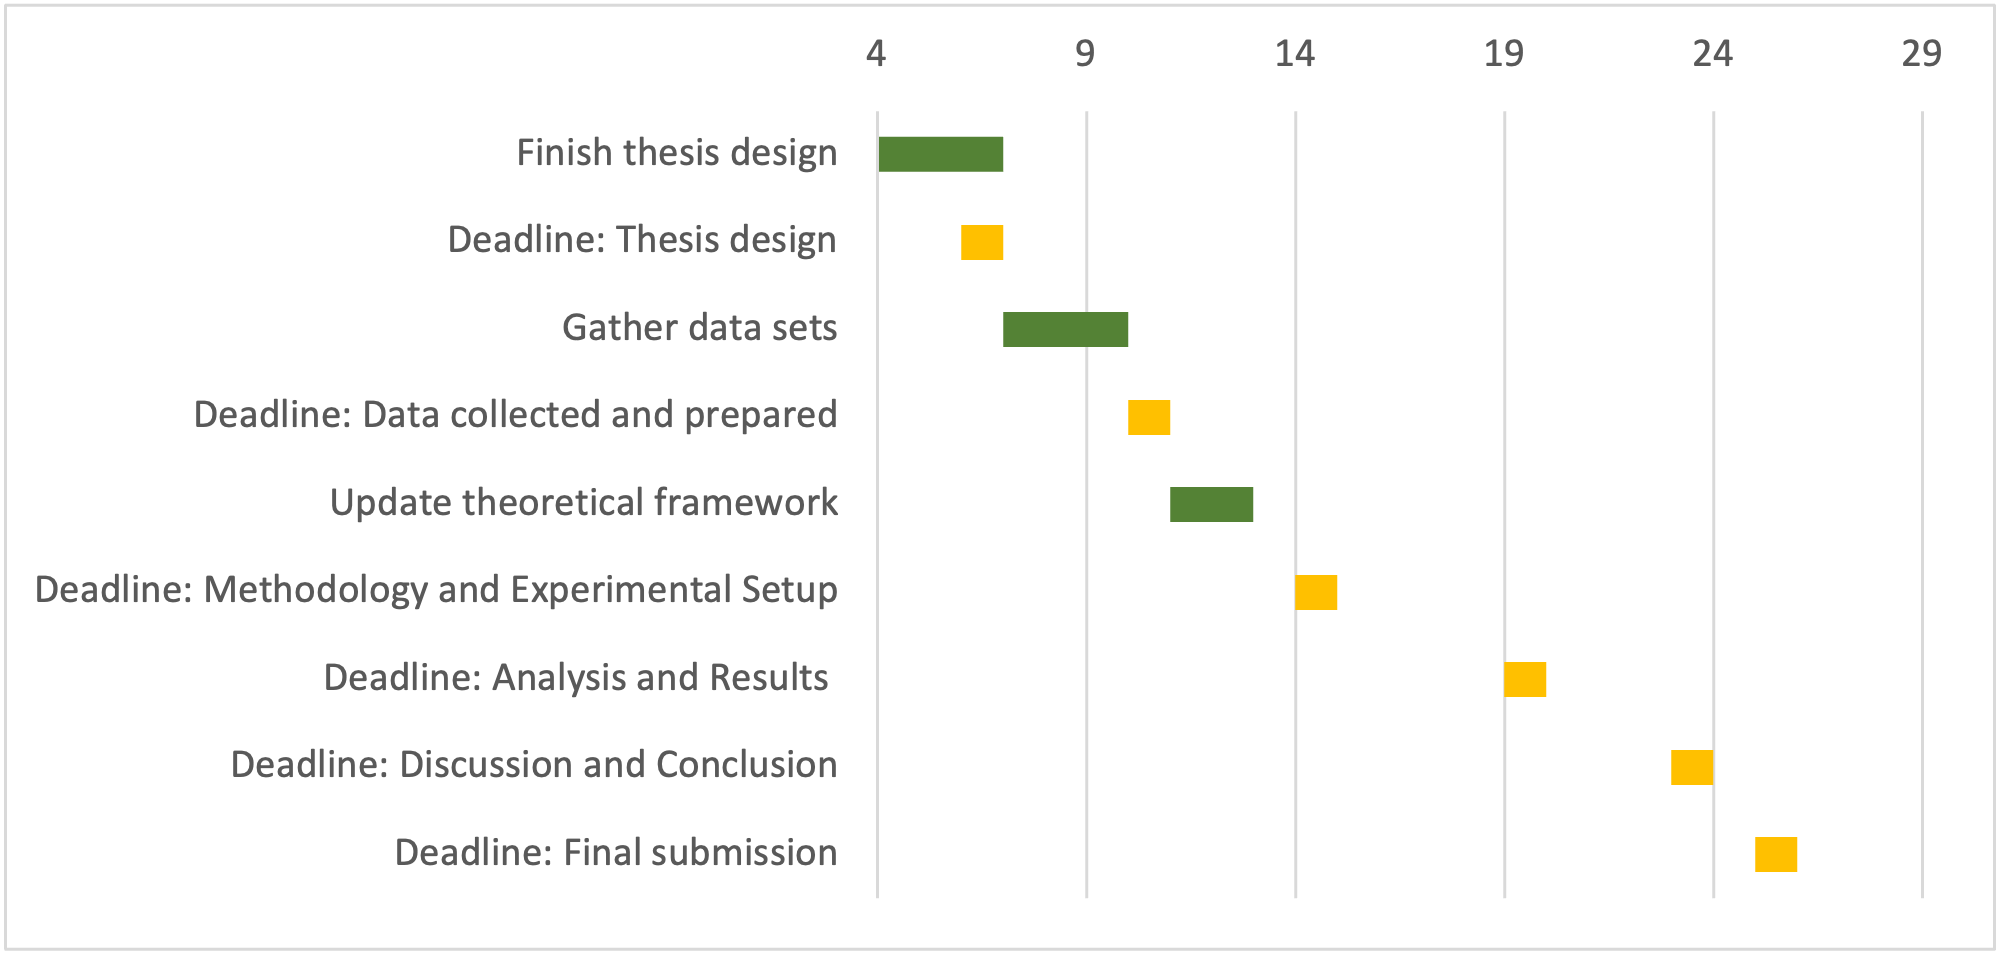
\includegraphics[width=\linewidth]{gantt-planning}
  \caption{Gantt chart on planning per calendar week.}
\end{figure}



%%
%% The acknowledgments section is defined using the "acks" environment
%% (and NOT an unnumbered section). This ensures the proper
%% identification of the section in the article metadata, and the
%% consistent spelling of the heading.


%%
%% The next two lines define the bibliography style to be used, and
%% the bibliography file.
\bibliographystyle{ACM-Reference-Format}
\bibliography{sample-base}

%%
%% If your work has an appendix, this is the place to put it.
\appendix


\end{document}
\endinput
%%
%% End of file `sample-lualatex.tex'.
